\documentclass[utf8,xcolor=table]{beamer}

\usepackage[T2A]{fontenc}
\usepackage[utf8]{inputenc}
\usepackage[english,russian]{babel}
%\usepackage{tikz-uml}
\usepackage{minted}

\mode<presentation>{
	\usetheme{CambridgeUS}
}

\renewcommand{\t}[1]{\ifmmode{\mathtt{#1}}\else{\texttt{#1}}\fi}

\title{Редактор схем с распознаванием}
\author{Егор Суворов}
\institute[CSCenter]{Практика, осень 2014\\Куратор: Евгений Линский}
\date[18.12.2014]{Четверг, 18 декабря 2014 года}

\setlength{\arrayrulewidth}{1pt}

\begin{document}

\begin{frame}
\titlepage
\end{frame}

\begin{frame}[t]{Постановка задачи}
  Мотивация: оцифровка рисуемых схем в процессе рисования,
  чтобы был сразу виден результат.

  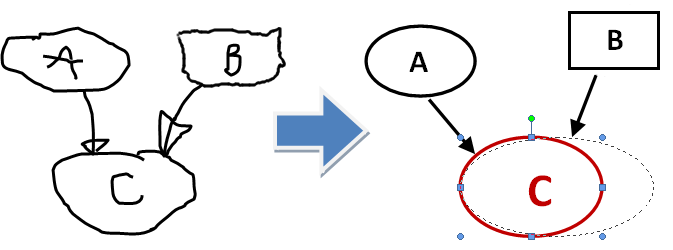
\includegraphics[width=\textwidth]{problem}
  \begin{itemize}
  \item~<<Умное перо>> для рисования векторных схем
  \item Распознавание фигур, соединений, жестов
  \item Автоматическая структуризация схемы
  \item Экспорт в SVG
  \end{itemize}
\end{frame}

\begin{frame}[t]{Модель}
  \begin{itemize}
  \item Схема "--- это набор фигур
  \item Фигура может быть:
    \begin{itemize}
    \item Отдельной: отрезок, стрелка, прямоугольник, эллипс
    \item Зависеть от положения других: отрезок, соединяющий две фигуры
    \end{itemize}
  \item Циклические зависимости невозможны
  \item Объекты класса <<фигура>> изменяемы
  \item Методы фигуры "--- только геометрические: пересчёт положения, расстояние до точки
  \item Отрисовкой занимается отдельный класс
  \end{itemize}
\end{frame}

\begin{frame}[t]{Алгоритм распознавания}
  Жест на области рисования "--- последовательность точек, \textit{трек}.
  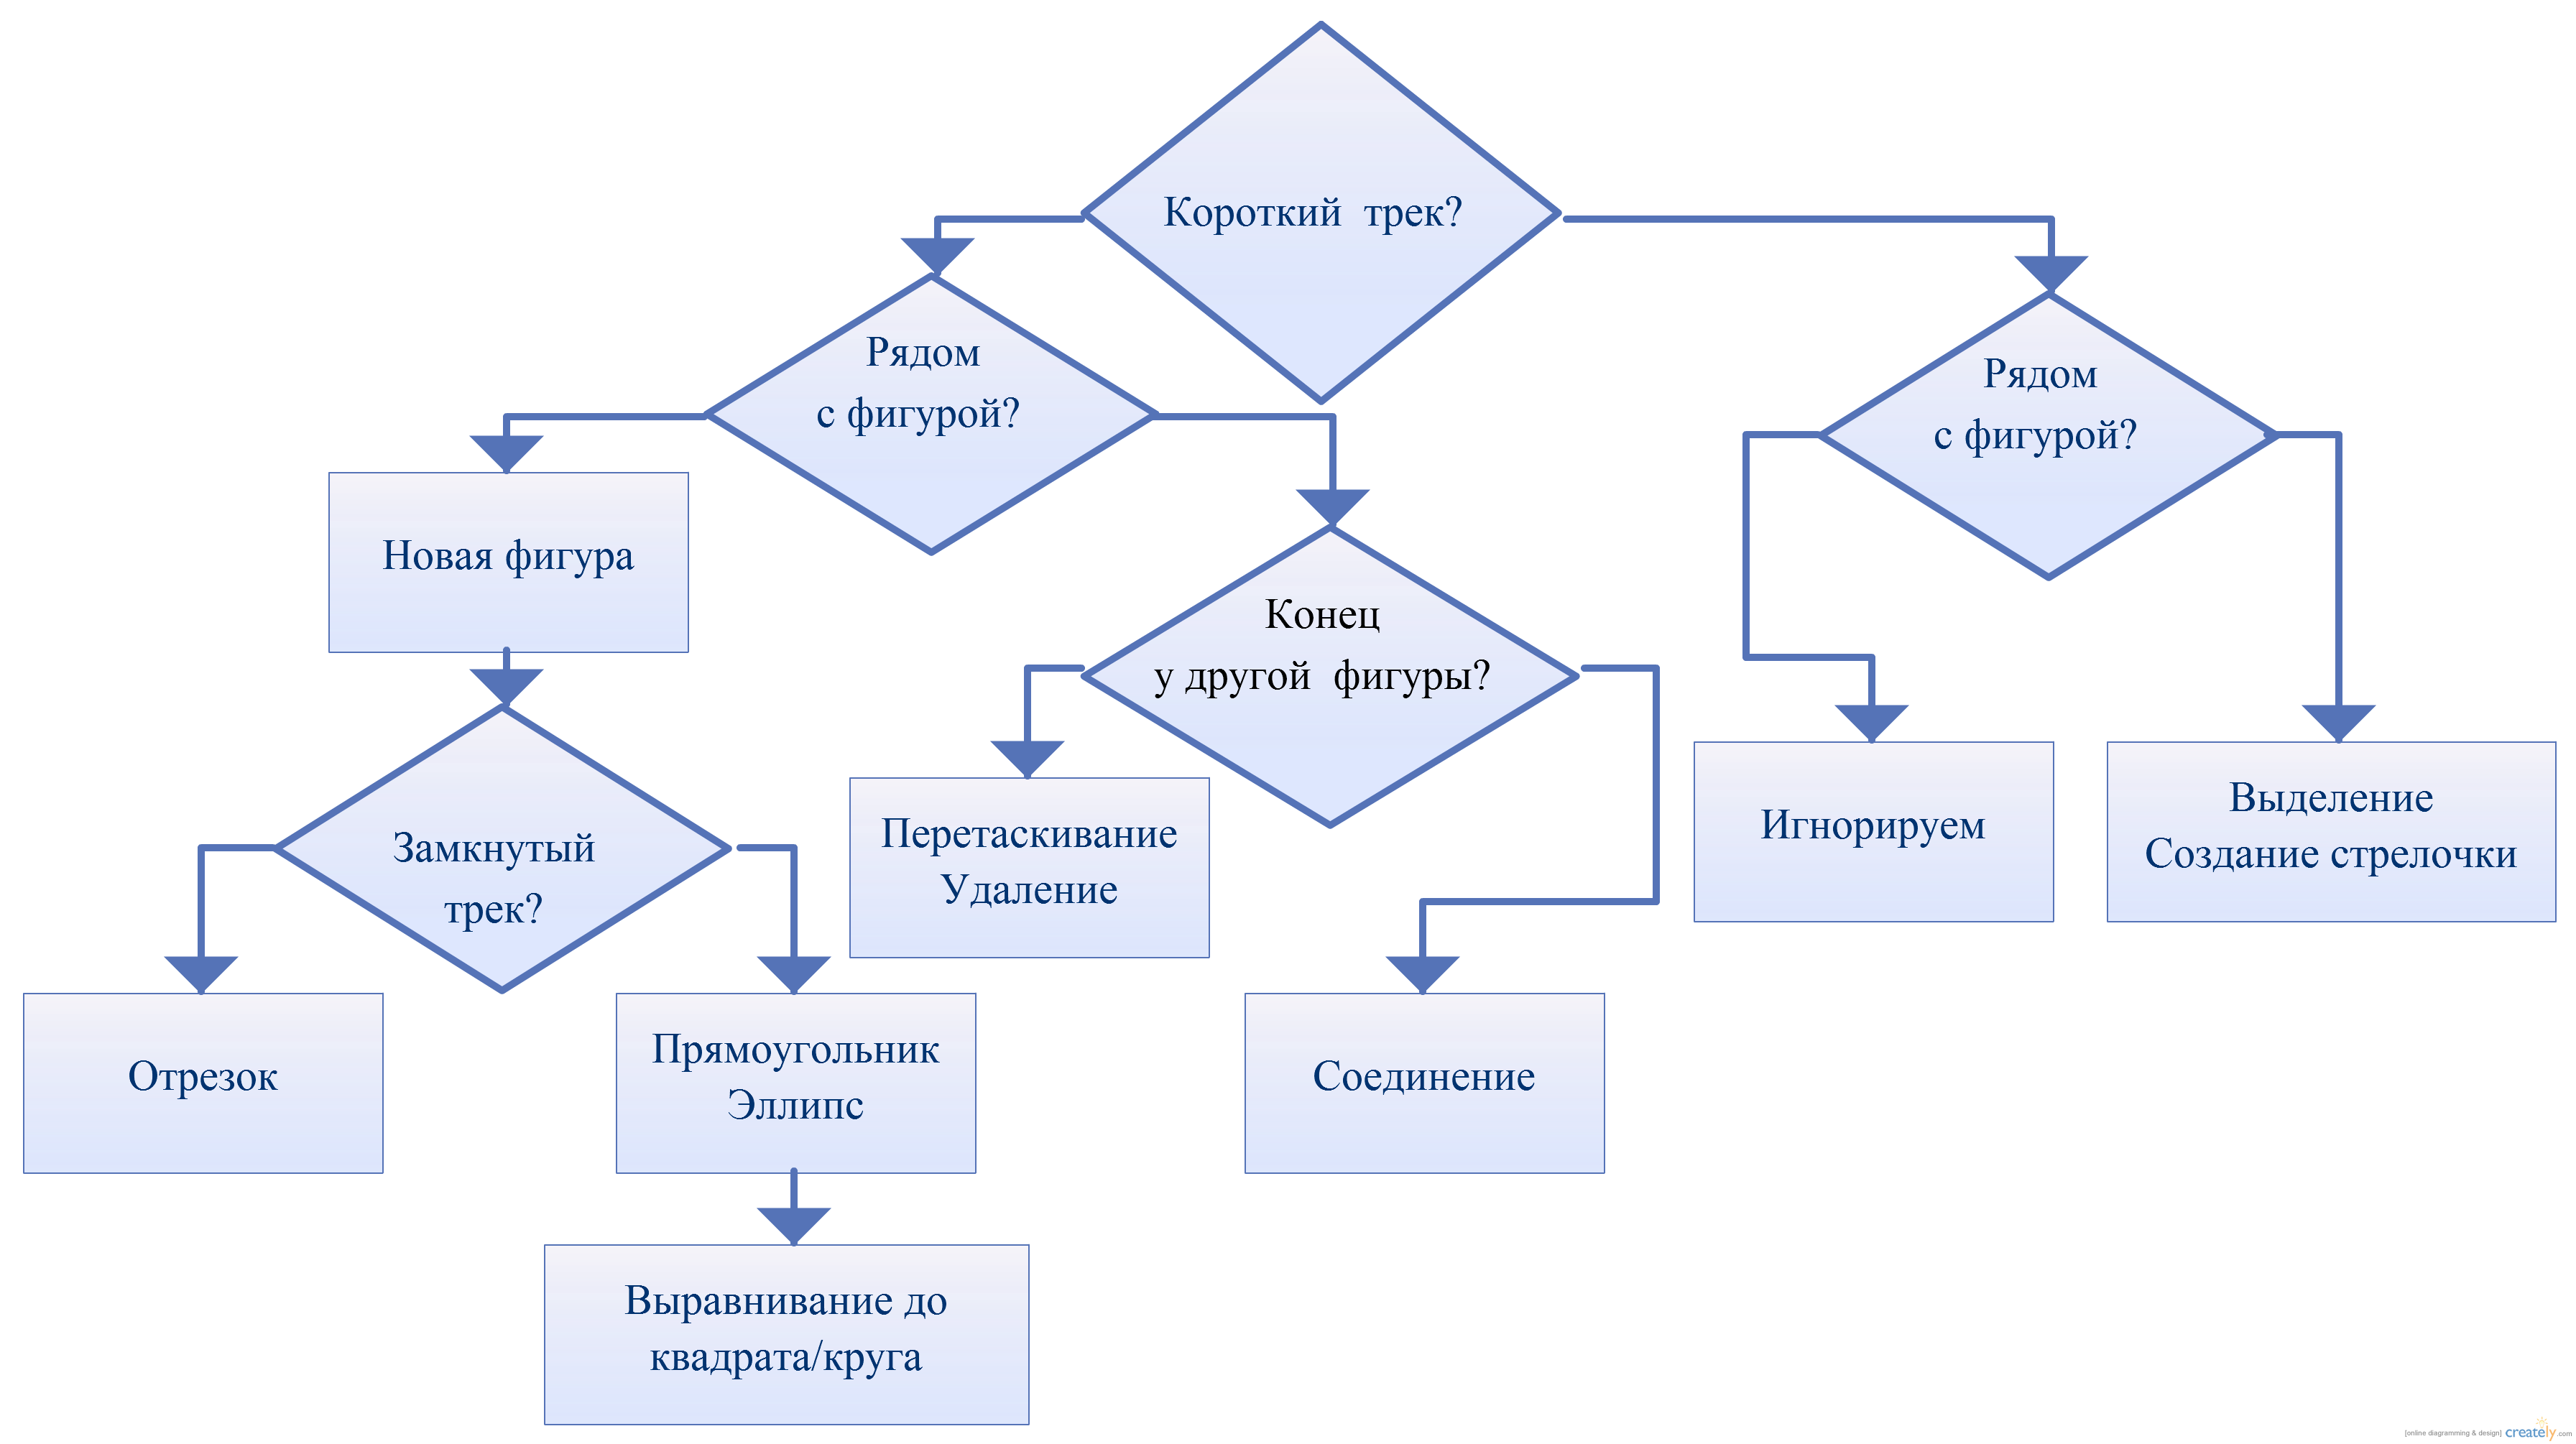
\includegraphics[width=\textwidth]{algo_schema}
\end{frame}

\begin{frame}[t]{Технические подробности}
  \begin{itemize}
  \item Написано на C++11 и Qt5, последний используется для UI и тестов, работает на Windows/Linux
  \item Разделены понятия <<точка фигуры>> и <<точка на экране>>
  \item Вместо указателей используется \t{std::shared\_ptr}
  \item Все фигуры наследуются от класса \t{Figure} и везде передаются по указателю
  \item Модель "--- это список фигур
  \item Каждая фигура хранит тех, от кого зависит и может обновляться по запросу
  \item Используется шаблон <<Visitor>> для:
    \begin{itemize}
    \item I/O модели через потоки \t{std} (собственный текстовый формат)
    \item Экспорт в SVG
    \item Отрисовка
    \end{itemize}
  \item На \t{qtest} написаны тесты на некоторые геометрические вычисления
  \end{itemize}
\end{frame}

\begin{frame}[t]{Уже сделано}
  \begin{columns}[T]
  \begin{column}{.6\textwidth}
    \begin{itemize}
    \item Распознавание:
      \begin{itemize}
      \item Прямоугольник, эллипс, отрезок
      \item Жесты удаления и перетаскивания
      \item Соединение фигур
      \end{itemize}
    \item Сохранение в свой формат
    \item Экспорт в SVG
    \item Real-time результат распознавания
    \item Undo
    \end{itemize}
  \end{column}
  \begin{column}{.4\textwidth}
    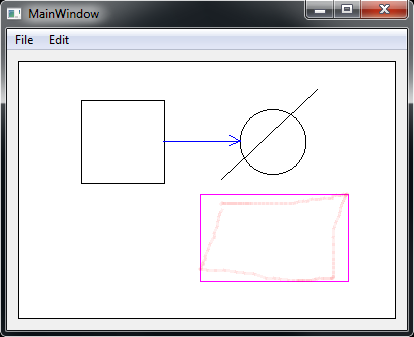
\includegraphics[height=3.5cm]{demo_scr}
  \end{column}
  \end{columns}
\end{frame}

\begin{frame}[t]{Планы}
  \begin{itemize}
  \item Добавление текста на схему
  \item Масштабирование и прокрутка в процессе редактирования
  \item Автоматическое выравнивание фигур, исходя из их типов и соединений:
    \begin{itemize}
    \item В дерево
    \item В блок-схему
    \item В граф
    \end{itemize}
  \item Новые типы фигур и жестов, улучшение отзывчивости
  \item Оптимизация производительности (при необходимости)
  \end{itemize}
\end{frame}

\begin{frame}[t]{Ссылки}
  \begin{itemize}
  \item \href{mailto:egor_suvorov@mail.ru}{\t{egor\_suvorov@mail.ru}}
  \item \href{http://github.com/cscenter/manugram/}{\t{github.com/cscenter/manugram}}
  \end{itemize}
\end{frame}

\end{document}
